\chapter{基于多通道模型引入上下文的情感识别}
\label{cha:exp_context_emo}

\section{本章引论}

在面向短文本的情感识别场景,有时候仅凭一段文本的内容可能无法完全理解发言者想表达的内容。考虑在一个甲乙两人对话的场景中,甲说“彼此彼此!”,我们可以认为甲表达了和乙相同的想法,但我们无法确认甲表达的情感。假如乙原本说“庆喜庆喜!”,那么可以认为甲也在表示祝贺,表达的是一种正面的情感。但假如乙原本说的是“你也不过如此!”,那么可以为甲在表示不满,表达的是一种负面的情感。因此在情感识别中,一些研究会考虑引入上下文信息作为辅助以提高识别性能。譬如Zahiri和Choi\cite{Zahiri2017Emotion}在研究电视剧剧本中每句台词的情感识别时,就引入了每句台词前的有限句台词作为上下文信息。Kunwoo等人\cite{hazarika2018conversational}在面向两人对话的情感识别研究中,同样引入了当前发言之前的有限段对话作为上下文信息。然而这些研究工作对上下文的建模方式都有所不同,如在Zahiri和Choi\cite{Zahiri2017Emotion}的研究中,一段剧本可能涉及多个角色,但在他们的模型中并没有考虑上下文中每句台词对应的角色,而在Kunwoo等人\cite{hazarika2018conversational}的研究中,由于对话过程只涉及两个人,在他们的模型中就区分了上下文中不同发言者说的话。对于不同场景下,如何在算法建模中引入上下文信息始终没有一种固定的方法,这也是因为不同类型的上下文包含的信息不同,对应具体的问题,我们依然需要进行针对性的模型设计。

国际比赛SemEval-2019的任务三\cite{SemEval2019Task3}则是旨在促进引入上下文的文本情感识别研究,比赛要求参赛者开发一个情感识别系统,对三轮对话中最后一轮发言表达的情感进行分类,给定的四个情感类别包括:开心、悲伤、愤怒、其他。为此我们提出了一个多通道模型,以引入作为上下文的前两轮对话。本章节中我们将基于SemEval-2019的任务三进行实验,采用比赛组织者提供的训练数据和测试数据,并透过和其他参赛系统进行比较来评估我们系统的识别性能。

本章的内容安排如下。在章节~\ref{sec:exp_context_emo_format}中,我们会首先给出当前问题的形式化表示。在章节~\ref{sec:exp_context_emo_data}中我们再对具体实验数据进行观察,分析给定数据集中各个情感类别的分布情况以及其文本特征等。在章节~\ref{sec:exp_context_emo_framework}将给出我们针对当前问题提出的多分类器分层识别算法,以及组成该最终识别系统的多通道分类模型。最后在章节~\ref{sec:exp_context_emo_exp},我们会给出实验的细节,以及对实验结果进行分析。

\section{形式化表示}
\label{sec:exp_context_emo_format}

在本章中,我们将研究面向三轮对话的情感识别,以下我们对应章节~\ref{sec:global_problem_analysis}给出此问题的形式化表示。给定一个情感类别集合$C$,对于一个三轮对话的集合$S$,其中任意一个元素$s$可以表示为一个三元组$<t^1, t^2, t^3>$,三元组中的元素依次对应每轮发言的文本内容。而在上下文为$b=<t^1, t^2>$的情况,最后一轮发言$t^3$所表达的情感属于唯一一种情感类别$c \in C$。又给定一个词集合$W$,对任意一轮发言的文本$t^j, j=1,2,3$,经过文本预处理后可以表示为一个长度为$L^j$的词序列 $w^j = <w^j_1, w^j_2, ..., w^j_{L^j}>, w^j_i \in W, i \in [1, L^j]$。那么我们的目标是找出一个映射关系$f$,使得$c=f(w^3, <w^1, w^2>)$。

\section{实验数据}
\label{sec:exp_context_emo_data}

我们的实验采用SemEval-2019的任务三提供的数据集,其中每个样本对应一个三轮对话以及第三轮发言的情感标签,第一轮为用户甲的发言,第二轮为用户乙对第一轮的回复,第三轮为用户甲对第二轮中用户乙的回复。情感标签对应四个情感类别中的其中一种:开心、悲伤、愤怒、其他。表~\ref{tab:semeval_2019_task3_data}显示数据集各类别样本数量分布,表~\ref{tab:semeval_2019_task3_sample}为语料中各个类别对应的样本例子。

\begin{table}[htb]
  \centering
  \begin{minipage}[t]{0.8\linewidth}
  \caption{情感识别各类别样本数量分布}
  \label{tab:semeval_2019_task3_data}
    \begin{tabularx}{\linewidth}{X|XXXX}
    \toprule[1.5pt]
    数据集 & 其他 & 开心 & 悲伤 & 愤怒 \\  
    \hline
    训练集 & 14948 & 4243 & 5463 & 5506 \\
    验证集 & 2338 & 142 & 125 & 150 \\
    测试集 & 4677 & 284 & 250 & 298 \\
    \bottomrule[1.5pt]
    \end{tabularx}
  \end{minipage}
\end{table}

\begin{table}[]
  \centering
  \begin{minipage}[t]{0.7\linewidth}
  \caption{各情感类别对应的三轮对话例子}
  \label{tab:semeval_2019_task3_sample}
  \begin{tabularx}{\linewidth}{c|l}
  \toprule[1.5pt]
   类别 & 对话    \\
  \hline
  \multirow{3}{*}{开心} 
    &   (第一轮)用户甲: live in uttra khand \\
    &   (第二轮)用户乙: ohh nice! love that place! \\
    &   (第三轮)用户甲: 
\includegraphics[height=1.5\fontcharht\font`\B]{img/emoji/lol.png}
\includegraphics[height=1.5\fontcharht\font`\B]{img/emoji/lol.png} \\
  \hline
  \multirow{3}{*}{悲伤} 
    &   (第一轮)用户甲: Not coz of you  \\
    &   (第二轮)用户乙: why? Tell me  \\
    &   (第三轮)用户甲: :( My girlfriend left me \\
  \hline
  \multirow{3}{*}{愤怒} 
    &   (第一轮)用户甲: He is over me \\
    &   (第二轮)用户乙: so YOU say \\
    &   (第三轮)用户甲: I just hate him \\
  \hline
  \multirow{3}{*}{其他} 
    &   (第一轮)用户甲: degreee \\
    &   (第二轮)用户乙: what degree \& where? \\
    &   (第三轮)用户甲: sryyy i really got to goo \\
  \bottomrule[1.5pt]
  \end{tabularx}
  \end{minipage}
\end{table}


在训练集上“其他”、“开心”、“悲伤”、“愤怒”四个类别的样本数量分布约为3:1:1:1 ,而在验证集和测试集上四个类别的样本数量分布约为22:1:1:1 。可见在验证集和测试集上“其他”一类的样本数量要远高于其他三个类别,和训练集相比其样本占比也相对较高,而另外三个类别的样本数量在各个数据集上则大致相同。

在比赛的最终测试阶段,训练集和验证集均已公布情感标注并且被允许用于模型训练,因此我们结合了原本的训练集和验证集作为我们的训练数据。

\subsection{文本长度}

我们对数据集的文本进行分词后统计了各类别样本的单词数量分布,以下简称为文本长度。表\ref{fig:context_emo_train_class_len}显示在训练集上各情感类别的样本在每轮发言的文本长度分布,可以看出在每轮发言中,不同类别样本的文本长度分布大致相同。虽然第一轮和第三轮的样本中最长的文本分别达到146个词和74个词,但各轮样本的文本长度大部分在22个词以内,约为前一章实验数据中样本文本长度的一半。

\begin{figure}[h]
  \centering%

  \begin{minipage}{\linewidth}

  \subcaptionbox{第一轮\label{fig:context_emo_train_class_len_0}} %[3cm] 
    {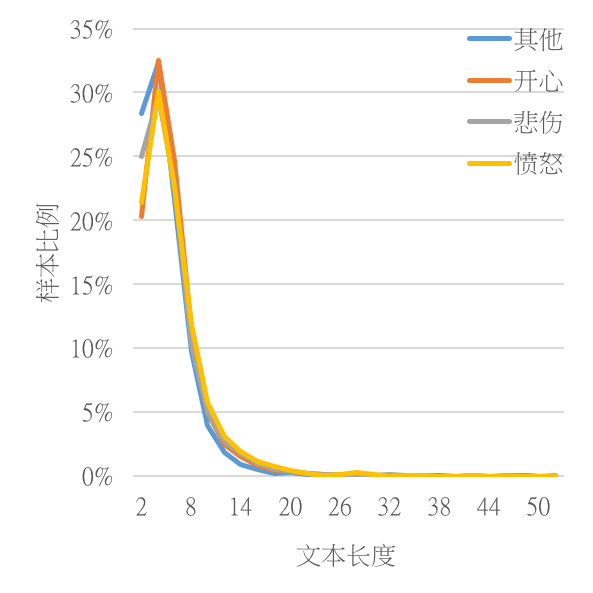
\includegraphics[height=8cm]{img/semeval2019_task3_train_0_class_len.png}}%
  %\hspace{em}%
  \subcaptionbox{第二轮\label{fig:context_emo_train_class_len_1}}
      {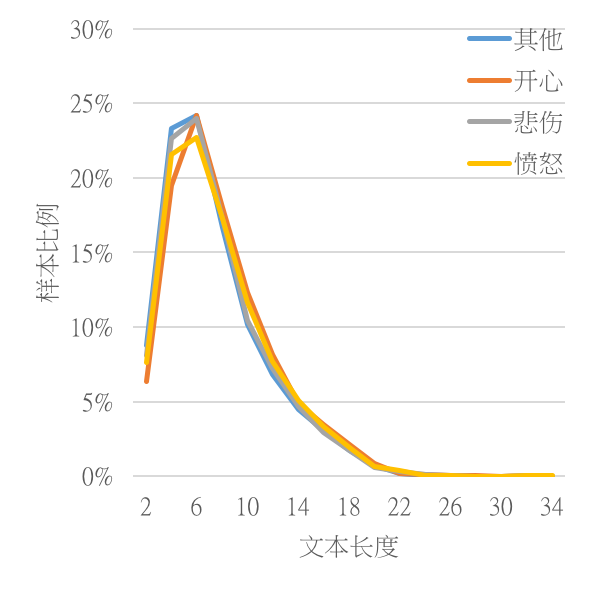
\includegraphics[height=8cm]{img/semeval2019_task3_train_1_class_len.png}}

  \end{minipage}
  \vspace{0.5cm} 

  \subcaptionbox{第三轮\label{fig:context_emo_train_class_len_2}}
      {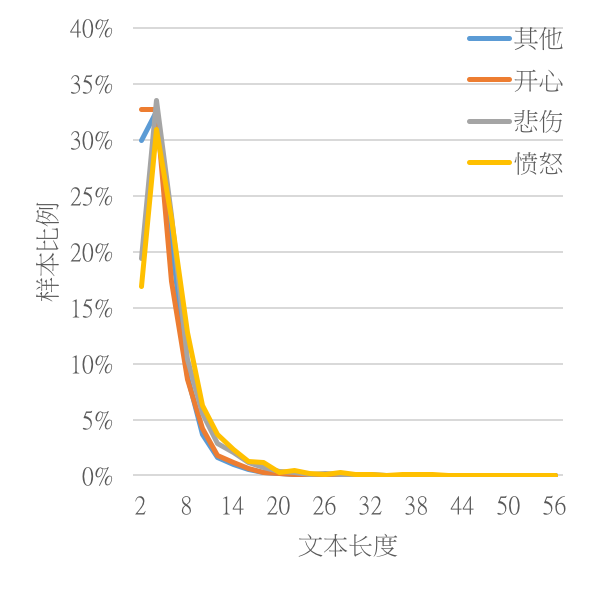
\includegraphics[height=8cm]{img/semeval2019_task3_train_2_class_len.png}}

  \caption{训练集上各情感类别的样本在每轮发言的文本长度分布}

  \label{fig:context_emo_train_class_len}
\end{figure}

\subsection{文本特征}
\label{ssec:exp_context_emo_data_text}

对于比赛中提供的数据集,比赛组织者并没有给出数据的具体来源,但经过人工观察后我们可以发现一些社交网络上常见的文本特征,其中出现频率较高的特征如下:

\begin{itemize}

\item 大量的缩略词使用,如“u”代替“you”,“y”代替“why”,“im”代替“I am”。

\item 出现在句子最前或最后的表情符,其中包括Unicode定义表情符(如
\includegraphics[height=1.5\fontcharht\font`\B]{img/emoji/lol.png})和由标点符号组成的表情符(如“:-D”)两类。

\item 一些在社交媒体平台上常见的、有别于正规英语的用法,如拼写错误、全大写字母的单词等,可以参考章节\ref{ssec:text_preprocess}描述的例子。

\end{itemize}

\subsection{各轮发言间的情感信息}
\label{ssec:exp_context_emo_multi_turn_analyse}

为了结合三轮对话中前两轮的发言来预测最后一轮发言的情感,我们需要观察各轮发言是否关最后一轮发言的情感有关,若有关的话各轮发言是否起着相同的作用。以下我们将采用数据集中的具体例子说明我们对语料的观察和理解。

首先,对于三轮发言中两个用户的情感,我们发现用户甲和用户乙表达的情感可能截然不同,参考以下例子:

\makebox[4 cm]{(第一轮)用户甲:} yes yay fun\par
\makebox[4 cm]{(第二轮)用户乙:} are not you joining us? :( \par
\makebox[4 cm]{(第三轮)用户甲:} yes\par

用户甲在最后一轮发言的情感标签为“开心”,而第一轮发言在字面意思上同样偏向正面。而对于用户乙在第二轮的发言,根据上下文意思和最后文本末尾的“:(”,我们可以推断用户乙的情感为“伤心”。可见三轮对话中两个用户表达的情感可能不同甚至矛盾,因此用户甲的发言和用户乙的发言对识别第三轮发言的情感应起着不同的作用,第二轮中用户乙的发言甚至没有提示的作用。

另外对于用户甲,我们发现他在第一轮和第三轮中表达的情感也有可能不同,参考以下例子:

\makebox[4 cm]{(第一轮)用户甲:} not fine\par
\makebox[4 cm]{(第二轮)用户乙:} why? :'o \par
\makebox[4 cm]{(第三轮)用户甲:} tomorrow lab exam\par

用户甲在最后一轮发言的情感标签为“悲伤”,而在字面意思上,最后一轮发言的情感偏中性,只是在陈述“明天有考试”的事情,“悲伤”的情感提示主要来自用户甲在第一轮中表示自己的情况“不太好”,第三轮发言在解释“不太好”的原因。基于此例子可以认为,同为用户甲发言的第一轮在某此情况下对识别第三轮发言的情感起着决定性作用。再观察下面的例子:

\makebox[4 cm]{(第一轮)用户甲:} ohh sorry\par
\makebox[4 cm]{(第二轮)用户乙:} do not worry, you are not the first \par
\makebox[4 cm]{(第三轮)用户甲:} glad to hear\par

用户甲在最后一轮发言的情感标签为“开心”,对于用户甲在第一轮发言表达的情感,结合用户乙在第二轮的发言,可以认为用户甲在第一轮发言中表示对用户乙的同情,这与“开心”为不同的情感,而在用户乙发言后,用户甲的情感因为用户乙说的话而转换成“开心”。可见用户甲在第一轮和第三轮中表达的情感有可能不同,这种情感的转变可能由用户乙的发言造成,但无论具体原因是什么,用户甲在第一轮和第三轮中的发言对识别第三轮发言的情感应起着不同的作用。

再者,我们发现用户甲在第三轮发言中可能出现多于一种情感,参考以下例子:

\makebox[4 cm]{(第一轮)用户甲:} 
\includegraphics[height=1.5\fontcharht\font`\B]{img/emoji/laugh.png} yes yes \par
\makebox[4 cm]{(第二轮)用户乙:} :3 you seem like a happy person \par
\makebox[4 cm]{(第三轮)用户甲:} yes 
\includegraphics[height=1.5\fontcharht\font`\B]{img/emoji/lol.png} happy outside, 
\includegraphics[height=1.5\fontcharht\font`\B]{img/emoji/frown.png} sad inside \par

用户甲在最后一轮发言的情感标签为“悲伤”,而在文本上,第三轮发言的前半表现为正面情感,后半表现为负表情感,前后的情感不同。对于当第三轮发言中出现两种情感时情感标签以何者为准,比赛组织者并没有给出细节的说明,但对语料的观察可以发现普遍以后面出现的情感为主。

最后总结我们对语料的观察,我们发现三轮发言对识别第三轮发言的情感应起着不同的作用。当第三轮发言有明显的情感表达,我们可以无视前两轮的发言得出识别结果。当第三轮发言表达的情感较隐晦或偏中性,需要参考同为用户甲发言的第一轮的信息。第二轮发言对第三轮发言的情感识别未有明显的提示作用。

\begin{figure}[H]
  \centering
  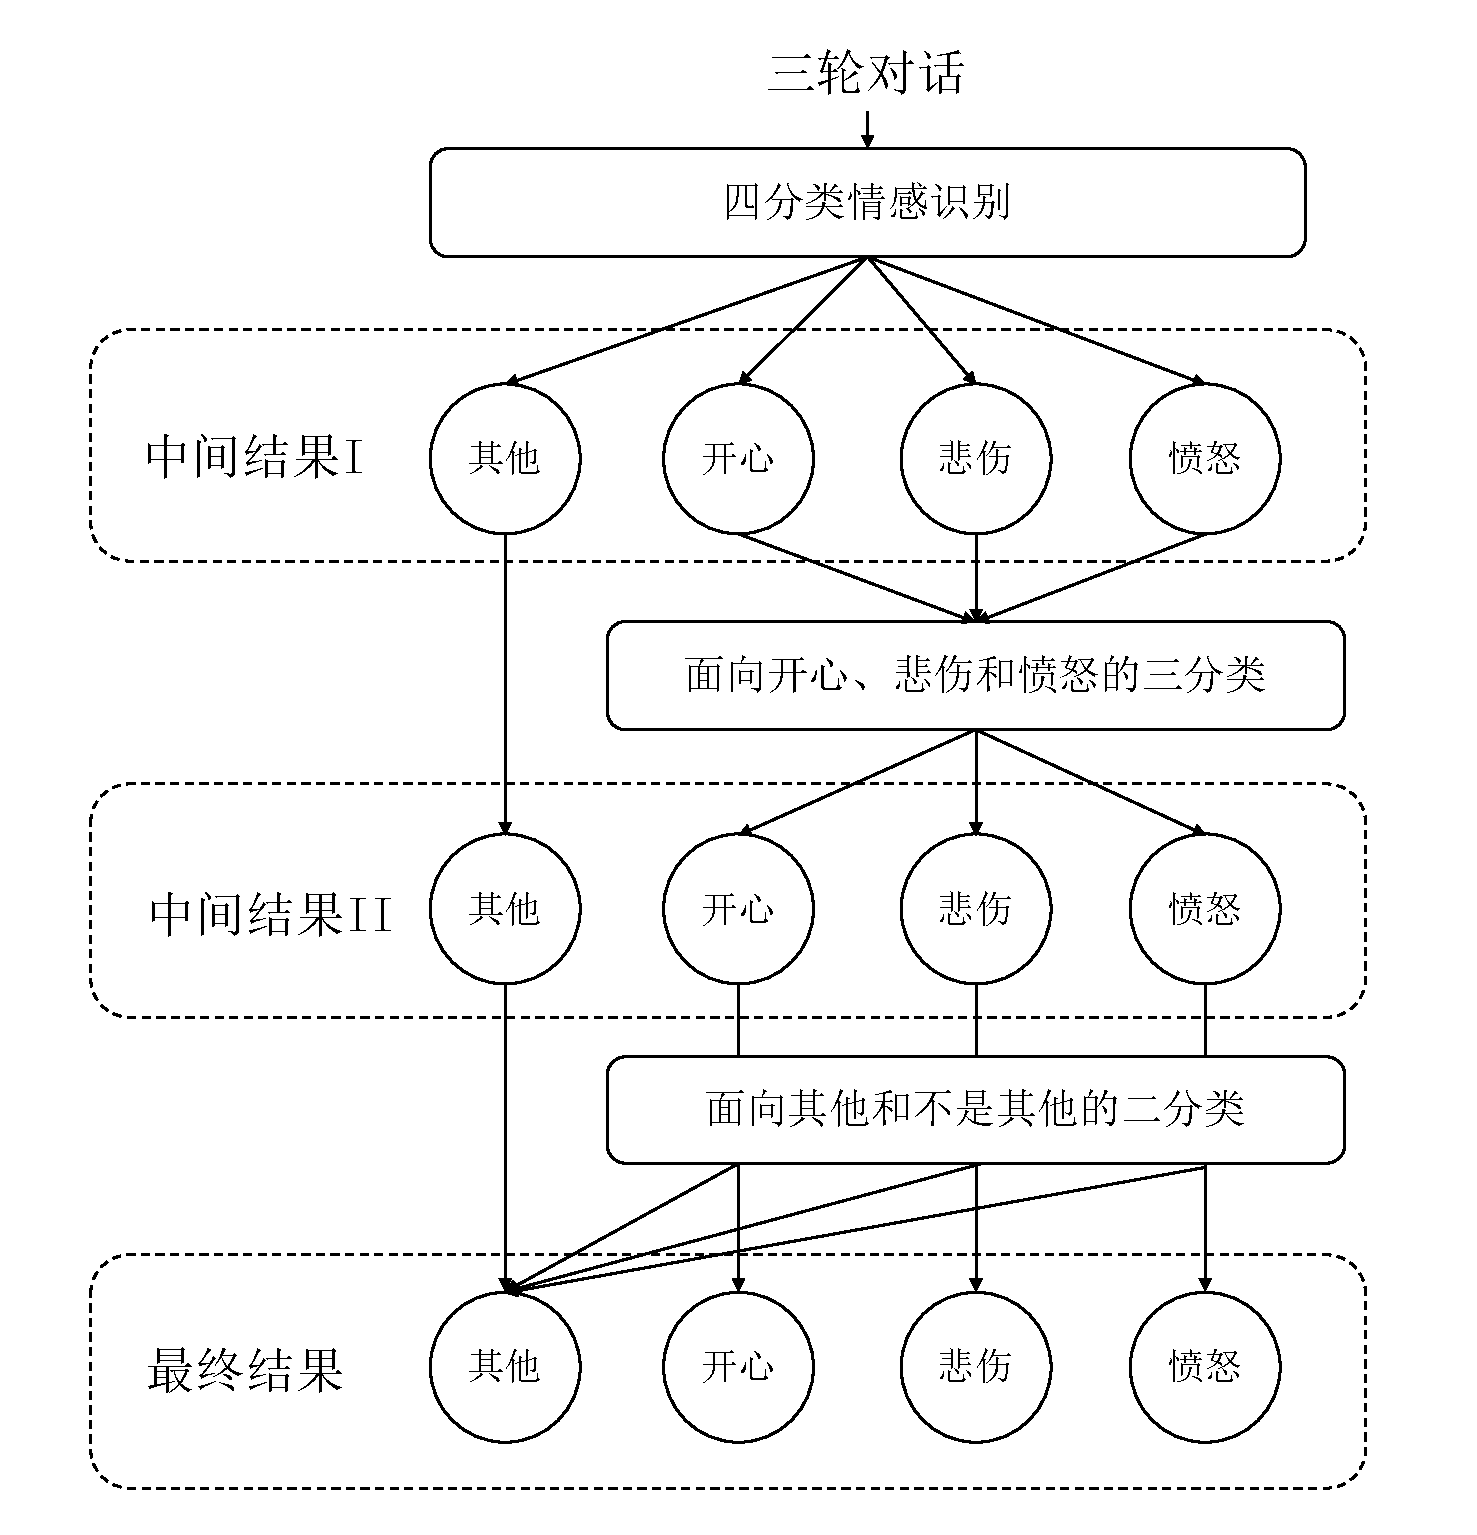
\includegraphics[width=0.9\textwidth]{img/context_emo_system.pdf}
  \caption{面向四分类情感识别的多分类器分层识别算法}
  \label{fig:context_emo_system}
\end{figure}

\section{框架设计}
\label{sec:exp_context_emo_framework}

同样地,我们提出了一个多分类器分层识别算法。对于原本的情感四分类问题,我们把它拆解成了以下三个子分类问题的叠加:

\begin{enumerate}

\item 原本的情感四分类问题。
\item “开心”、“悲伤”和“愤怒”三分类。
\item “其他”和“不是其他”二分类。

\end{enumerate}

对于每个子分类问题,我们分别准备其对应的分类器组,依次命名为第一、第二、第三组分类器,分别由$N_1$、$N_2$、$N_3$个分类器组成。那么对于三轮对话中最后一轮发言的情感识别,我们系统的决策过程如下:

\begin{itemize}

\item 首先由对应原四分类问题的第一组分类器进行多数投票,得出预测标签$Label^{1}_{MV}$,直接以它作为第一步的预测标签$Label_{I}$ 。以下把算法到这一步为止的判断结果称为中间结果I。

\item 第二步,由面向“开心”、“悲伤”和“愤怒”三分类的第二组分类器进行多数投票,得出预测标签$Label^{2}_{MV}$,若超过$thr_{2}$分类器投票投给$Label^{2}_{MV}$且第一步的预测标签$Label_{I}$为“其他”以外的三种情感类别之一,则把预测结果修改为$Label^{2}_{MV}$,否则保持不变,以此得出第二步的预测标签$Label_{II}$。以下把算法到这一步为止的判断结果称为中间结果II。

\item 最后一步,由面向“其他”和“不是其他”二分类的第三组分类器给出投票结果,若超过$thr_{3}$个分类器投票给“其他”且第二轮的预测标签$Label_{II}$不是“其他”,则把预测标签修改为“其他”,否则保持不变,以此得出第三步的预测标签$Label_{III}$,同时作为整个算法对第三轮发言最终的情感识别结果。

\end{itemize}

整个决策过程可以分成两大部分。第一部分的目的是初步完成对第三轮发言的四分类情感识别,对应上述三步决策中的第一步。第二部分的目的是基于第一部分的初步识别结果逐步进行修正,每一步只关注一个子分类问题,对应上述三步决策中的后两步。其中第二步进行“开心”、“悲伤”和“愤怒”的三分类,目的在于调整三个类别之间的识别结果。而在最后一步进行“其他”和“不是其他”二分类,但特别地不是取多数投票,而是只要超过$thr_{3}$个分类器投票给“其他”即把识别标签改成“其他”,目的在于提高系统对“其他”一类的召回率。

其中对于每个子分类问题,我们都采用了我们提出的多通道分类模型框架,如图\ref{fig:context_emo_cls_framework}所示,每个子分类器的输入为三轮对话对应的词序列$\{w^1, w^2, w^3\}$。根据在章节\ref{ssec:exp_context_emo_multi_turn_analyse}中的分析,我们认为三轮发言对识别第三轮发言的情感识别起着不同的作用,因此三轮发言对应的词序列分别进入不同的通道。每个通道的结构相同,第一步都是把词序列转换成对应的词嵌入向量序列,作为特征编码器的输入。此处特征编码器的设计与章节\ref{sec:exp_irony_det_framework}中的相同,目的是把单轮发言对应的词向量序列转换成固定长度的特征向量,以此得出该轮发言的特征向量。为了简化,三个通道的特征编码器采用相同的模型,但考虑到每轮发言对第三轮情感有关的特征可能不同,三个通道的模型各自采用不同的权重。分别得出三轮发言的特征向量后我们需要结合这些特征来识别第三轮的情感类别,此处我们直接把三个向量拼接成一个向量,作为概率预测器的输入。此处概率预测器的设计与章节\ref{sec:exp_irony_det_framework}中的相似,但实现上采用了两层的全联接层,第一层的激活函数为线性整流函数(Rectified Linear Unit, ReLU),而第二层的激活函数依然为$Softmax$,以得出各个情感类别的概率分布。

考虑到对于不同情感类别的语言特征不同,各个模型的建模能力也会有所不同。所以对于每个子分类问题,我们会分别比较各个模型的性能,以求在子分类问题上达到尽可能好的识别性能。

\begin{figure}[H]
  \centering
  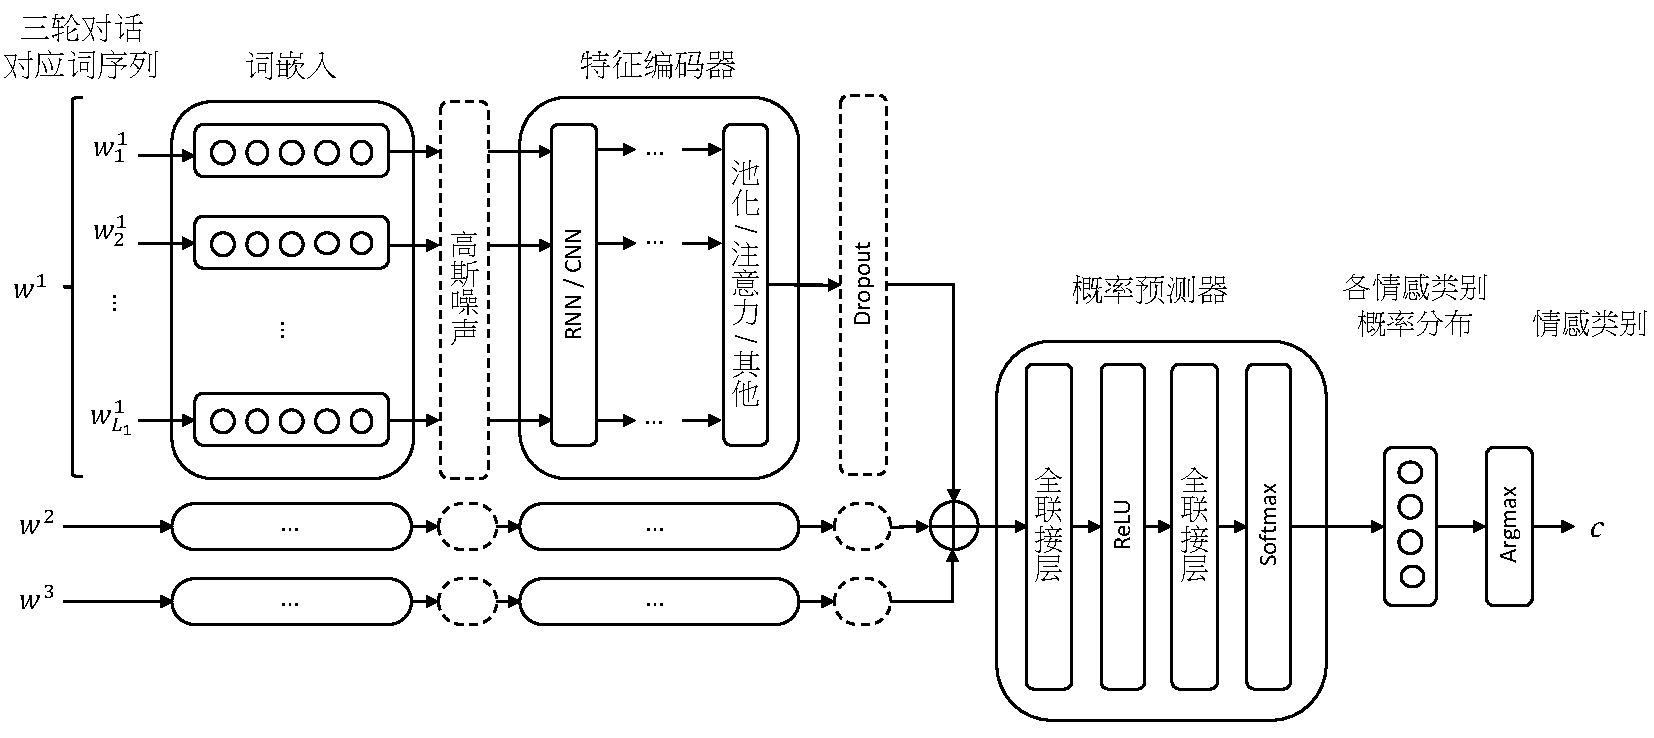
\includegraphics[width=\textwidth]{img/context_emo_cls_framework.pdf}
  \caption{面向三轮对话情感识别的多通道分类模型框架}
  \label{fig:context_emo_cls_framework}
\end{figure}

\section{实验与分析}
\label{sec:exp_context_emo_exp}

\subsection{数据预处理}

基于我们在章节\ref{ssec:exp_context_emo_data_text}中对样本文本的观察,我们依次采取了以下数据预处理手法

\begin{itemize}

\item 对于全字母大写的文本段,在该段文本的前后添加“<allcap>”和“</allcap>”示意。如“YAYYYY”替换成序列“<allcap>”、“yayyyy”、“</allcap>”。

\item 对于重复次数大于等次三次的标点符号,以“<repeated>”示意,如“!!!”替换成序列“!”、“<repeated>”,表示“!”被多次重复,即时假设重复的具体次数和原微博的反讽类别无关。

\item 对于字母被故意重复的单词,以“<elongated>”示意,如“Noooooooo”替换成序列“No”、“<elongated>”,表示“No”中某一个或多个字母被多次重复,即假设被重复的字符和具体重复的次数和原微博的反讽类别无关。

\item 将数字串替换成“<num>”,将电话号码替换成“<phone>”,将日期和时间分别替换成“<date>”和“<time>”,将数字百分比替换成“<percentage>”,超链接替换成“<url>”,即假设其中的具体数值和原微博的反讽类别无关。

\item 对于由多个标点符号组成的表情符,我们将其替换成对应的情感标签,如将“:)”替换成“<happy>”,“:((”替换成“<sad>”。

\item 在完成以上处理后,对英文的大小写统一转换成小写。

\end{itemize}

具体实现和章节~\ref{ssec:exp_irony_det_text_preprocess}中的相同。

\subsection{评价指标}
\label{ssec:exp_context_emo_eval_metric}

按照国际比赛SemEval-2019任务三的设置,系统性能以针对“开心”、“悲伤”和“愤怒”三个情感类别的F1值(以下记为 $F_\mu$)作为识别系统性能的主要评价指标。其定义如下:

\vspace{-10mm}
\begin{equation}
\vspace{-2.5mm}
\begin{aligned}
  F_\mu &= \frac{2 \times P_\mu \times R_\mu}{P_\mu + R_\mu}
\end{aligned}
\end{equation}

其中 $P_\mu$ 和 $R_\mu$ 分别是针对“开心”、“悲伤”和“愤怒”三个情感类别的正确率和召回率,其定义如下:

\vspace{-10mm}
\begin{equation}
\vspace{-2.5mm}
\begin{aligned}
  P_\mu &= \frac{\sum\limits_{c \in C} TP_c}{\sum\limits_{c \in C}(TP_c + FP_c)} \\
  R_\mu &= \frac{\sum\limits_{c \in C} TP_c}{\sum\limits_{c \in C}(TP_c + FN_c)}
\end{aligned}
\end{equation}

其中 $C$对应情感类别集合\{开心,悲伤,愤怒\},$TP_c$表示被系统预测为类别$c$,且真实标签为类别$c$的样本数量;$FP_c$表示被系统预测为类别$c$,但真实标签不是类别$c$的样本数量;$FN_c$被系统预测为不是类别$c$,但真实标签为类别$c$的样本数量。

\begin{table}[htb]
  \centering
  \begin{minipage}[t]{0.55\linewidth}
  \caption{模型训练参数}
  \label{tab:exp_context_emo_model_param}
    \begin{tabularx}{\linewidth}{X|l}
    \toprule[1.5pt]
    参数 & 数值 \\
    \hline
    词向量维数 & 300 \\
    RNN内各隐藏层神经元数量 & 50 \\
    CNN卷积核大小 & 3 \\
    CNN过滤器数量 & 64 \\
    注意力机制的隐藏层神经元数量 & 50 \\
    概率预测器全连接层的神经元数量 & 32 \\
    高斯噪音的标准方差 & 0.1 \\
    Dropout比例 & 0.5 \\
    学习率初始值 & 0.005 \\
    学习率衰减系数 & 0.9 \\
    L2正则项权重 & 0.2 \\
    训练的迭代次数 & 200 \\
    训练的批大小 & 100 \\
    \bottomrule[1.5pt]
    \end{tabularx}
  \end{minipage}
\end{table}

\subsection{模型训练}
\label{ssec:exp_context_emo_model_training}

对于每个子分类问题,我们分别从完整的训练数据和测试数据中筛选出对应类别的样本作为实验数据。并采用相同的方法进行模型训练,训练参数如表~\ref{tab:exp_context_emo_model_param}所示,另外采用了一些训练策略如下:

\begin{itemize}

\item 对于涉及类别“其他”的子分类问题,我们在模型训练前会基于“其他”的每一个样本随机生成一个新的临时样本。生成方法是在三轮发言中随机选择一轮,再在该轮发言的文本中随机选择一个词删掉,以此模拟用户使用未被识别的单词或错拼词,得出一个“其他”的新样本。这使得模型对识别“其他”有更好的鲁棒性,但这会同时导致模型倾向于将更多不是“其他”的样本识别为“其他”。对于为什么只基于类别“其他”的样本生成新的临时样本,原因在于语料中类别为“其他”的三轮对话在忽略一个单词后并不会带来情感类别的变化。但对于类别“开心”、“悲伤”和“愤怒”,大部分样本仅以一个或几个单词表达其情感,若其中一个单词被删除会直接导致其情感表达的变化,为避免产生有误导性的临时样本,我们只基于类别“其他”的样本生成新的样本。

\item 对于训练数据,我们分别从各个类别的样本中随机选出90\%的样本作为训练集,剩余10\%的样本作为验证集,以保留各个类别的样本分布。在每一轮模型参数调整后,计算各组模型参数在验证集上的某个指标,经过有限轮迭代后,取在验证集上性能指标最优的网络参数作为该分类器的参数,以此避免在训练数据上过拟合。对第一组和第二组分类器,我们以“开心”、“悲伤”和“愤怒”的正确率$P_\mu$作为选择参数的指标,原因在于测试集中“开心”、“悲伤”和“愤怒”的样本占比要低于验证集(参考章节~\ref{sec:exp_context_emo_data}),这导致模型在测试集上会明显把较多“其他”的样本误判为这三种情感类别之一,正确率$P_\mu$的数值会明显下降,间接拉低了F1值$F_\mu$,故选择正确率$P_\mu$来确保模型的正确率$P_\mu$尽可能高。对于第三组分类器(“其他”和“不是其他”二分类),我们采用针对类别“其他”的正确率作为选择参数的性能指标,目的在于召回“其他”样本的同时尽可能保证其正确率。

\item 由于在我们的系统中,每个子分类问题由多个分类器经过投票给出识别结果,为了充分运用训练数据,在训练过程中每个分类器的验证集为独立随机筛选得出,一方面使得每个训练样本都有概率被用于某个分类器的模型训练,另一方面各个分类器的训练集不同,避免了对部分数据的过拟合。

\item 对于词嵌入层,我们利用了章节\ref{sssec:embedding}中Baziotis等人\cite{baziotis2018ntua}提供的词嵌入模型,直接用于初始化词嵌入层的参数。而对于词嵌入模型中未被覆盖的单词,若它在至少2个训练样本中出现,则为其随机生成词向量。在训练过程中,我们不对词嵌入层的参数进行调整。

\item 在参数训练阶段,我们对词嵌入层输出的词向量序列添加高斯噪音。由于词嵌入算法在原理上使得意思相似的单词投影到词嵌入空间中距离相近的点上,高斯噪音的添加相当于把原本的单词替换成近义词,使得模型能更好地理解近义词构成的语言模式,另一方面缓解过拟合的问题。在验证阶段和测试阶段,高斯噪音的标准方差被调整为零,即不起作用。

\item 在参数训练阶段,我们在特征编码器和概率预测器之间添加了Dropout层,以概率$p_{Dropout}$将特征编码器得出特征向量上的各位数值置为零,并对没有被置零的各位数值乘以常量 $\frac{1}{1-p_{dropout}}$。在验证阶段和测试阶段,Dropout层不起作用。

\item 对于模型训练的损失函数,我们以权重$l_2$加入了概率预测器中两个全联接层的权重(不包括偏移量)的L2正则项。

\end{itemize}

\subsection{实验结果与分析}

以下实验主要分成两大部分。第一部分是分析不同模型在不同子分类问题下的性能,根据章节\ref{sec:exp_context_emo_framework},我们的情感识别算法涉及以下多个子分类问题:区分“开心”、“悲伤”、“愤怒”和“其他”的四分类问题,区分“开心”、“悲伤”和“愤怒”的三分类问题、区分“其他”和“不是其他”的二分类问题。对于各个子分类问题,我们基于章节~\ref{sec:exp_context_emo_framework}中的子分类模型框架进行实验,透过采用不同配置了解不同模型对三轮对话的情感识别能力。

第二部分对我们提出的多分类器分层识别算法进行研究。一方面评估我们系统的整体性能水平,另一方面透过观察系统的中间结果分析算法中的每一步如何对算法的整体性能带来影响,从而解释算法设计的合理性。

\subsubsection{面向情感四分类的模型性能分析}
\label{sssec:exp_context_emo_0_base}

对于面向三轮对话的情感四分类问题,表~\ref{tab:exp_context_emo_0_result}和图~\ref{fig:exp_context_emo_0_result_bar}显示各个模型在测试集上的性能。注意表中的正确率、召回率、F1值为
针对“开心”、“悲伤”和“愤怒”的指标,对应比赛SemEval2019任务三关注的主要指标,即章节~\ref{ssec:exp_context_emo_eval_metric}中定义的$P_\mu$、$R_\mu$和$F_\mu$。

对于F1值,CNN达到最好的0.7437 ,其次是的BiGRU配合注意力机制和CNN配合注意力机制,两者和第一的CNN差距较大(约0.0384)。对于准确率,同样是CNN的数值最高(0.9245),第二和第三分别是BiGRU配合注意力机制和GRU配合注意力机制,同样地和CNN差距较大(约0.0102)。对于正确率,则是GRU配合注意力机制的性能最优(0.7330),其次的GRU和CNN和前者差距较小(仅0.0034)。对于召回率,第一位依然是CNN(0.7584),其次是CNN配合注意力机制,和前者差距约0.0156,第三的BiGRU配合注意力机制则和前两者差距较大(数值低于0.7)。

\begin{table}[htb]
  \centering
  \begin{minipage}[t]{\linewidth}
  \caption{面向情感四分类器的模型性能} 
  \label{tab:exp_context_emo_0_result}
    \begin{tabularx}{\linewidth}{X|llll}
    \toprule[1.5pt]
    & 准确率 & 正确率 & 召回率 & F1值 \\
    \hline
    CNN & \bf 0.9245 (1) & 0.7295 (3) & \bf 0.7584 (1) & \bf 0.7437 (1) \\ % f_cnn_ek_1554546621
    CNN+注意力机制 & 0.9071 (5) & 0.6574 (8) & 0.7428 (2) & 0.6975 (3) \\ % f_cnn_ek_1554545828
    \hline
    GRU & 0.9052 (8) & 0.7296 (2) & 0.5481 (9) & 0.6259 (9) \\ % f_gru_ek_1554462561
    GRU+注意力机制 & 0.9105 (3) & \bf 0.7330 (1) & 0.5974 (8) & 0.6583 (7) \\ % f_gru_ek_1554542220
    \hline
    BiGRU & 0.9067 (7) & 0.6598 (7) & 0.6923 (4) & 0.6757 (5) \\ % f_bgru_ek_1554465482
    BiGRU+注意力机制 & 0.9143 (2) & 0.7162 (4) & 0.6947 (3) & 0.7053 (2) \\ % f_bgru_ek_1554524728
    \hline
    LSTM & 0.9071 (5) & 0.6709 (6) & 0.6911 (5) & 0.6809 (4) \\ % f_lstm_ek_1554465719
    LSTM+注意力机制 & 0.8553 (10) & 0.2994 (10) & 0.2788 (10) & 0.2887 (10) \\ % f_lstm_ek_1554560984
    \hline
    BiLSTM & 0.8969 (9) & 0.6331 (9) & 0.6659 (6) & 0.6491 (8) \\ % f_blstm_ek_1554524691
    BiLSTM+注意力机制 & 0.9092 (4) & 0.7067 (5) & 0.6226 (7) & 0.6620 (6) \\ % f_blstm_ek_1554542227
    \bottomrule[1.5pt]
    \end{tabularx}
  \end{minipage}
\end{table}

\begin{figure}[H]
  \centering
  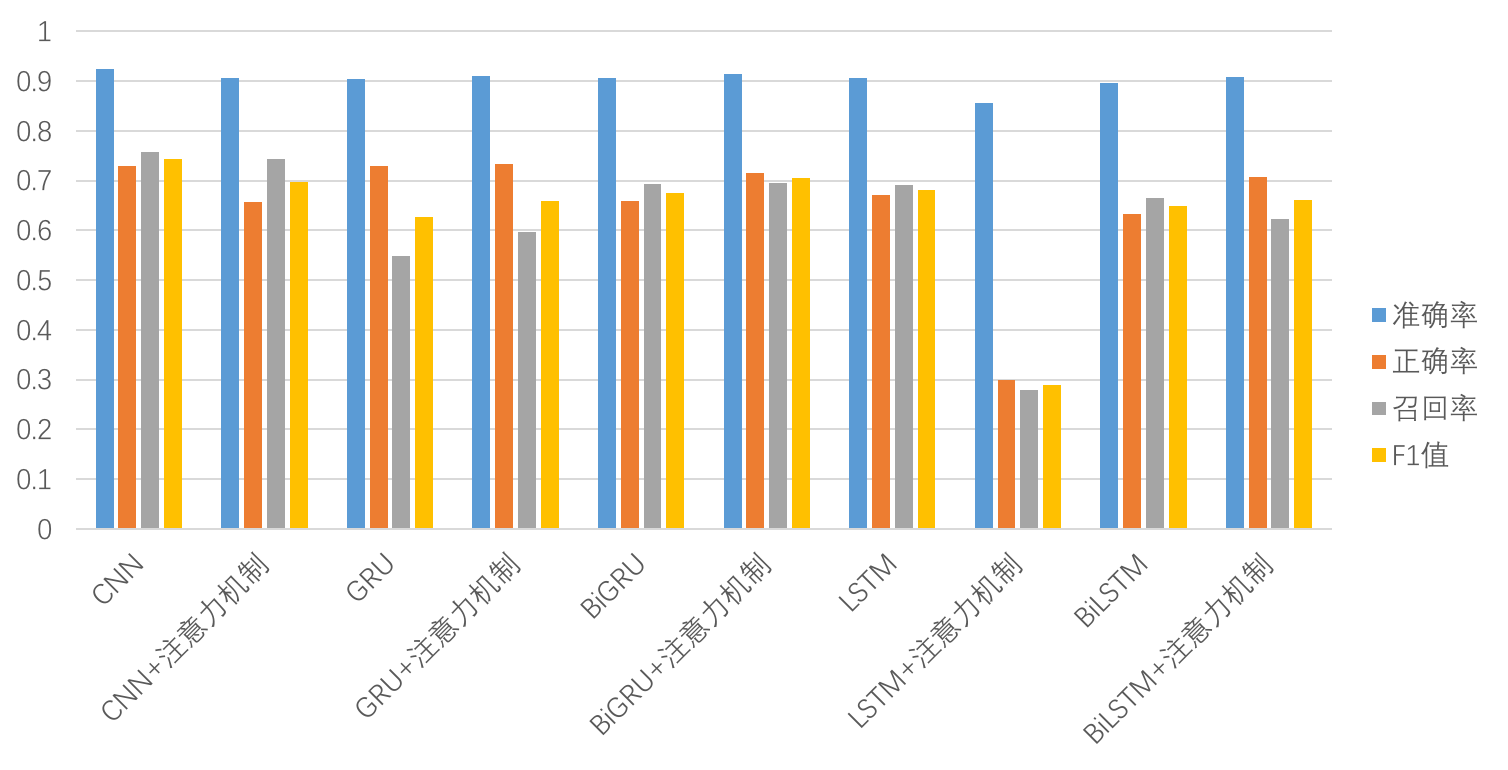
\includegraphics[width=\textwidth]{img/exp_context_emo_0_result_bar.png}
  \caption{面向情感四分类器的模型性能}
  \label{fig:exp_context_emo_0_result_bar}
\end{figure}

总的来说,CNN同时在F1值、准确率和召回率三项指标上达到了最好的性能,而正确率同样逼近最好的GRU配合注意力机制,可见CNN在此子分类问题上有显着较好的建模能力。另外值得注意的是LSTM配合注意力机制在各项指标中数据最低,其中正确率、召回率和F1值都远低于其他模型,经过检查后发现该模型在多次训练中都会忽略“开心”、“悲伤”和“愤怒”中的某个类。在排除算法实现有问题的可能性后,我们认为这是由于模型无法同时对四个类别的数据建模所致。

\subsubsection{面向“开心”、“悲伤”和“愤怒”三分类的模型性能分析}
\label{sssec:exp_context_emo_tri_base}

对于面向三轮对话的“开心”、“悲伤”和“愤怒”三分类问题,表~\ref{tab:exp_context_emo_tri_result}和图~\ref{fig:exp_context_emo_tri_result_bar}显示各个模型在测试集上的性能。注意表中的正确率、召回率、F1值同样对应章节~\ref{ssec:exp_context_emo_eval_metric}中定义的$P_\mu$、$R_\mu$和$F_\mu$。

\begin{table}[htb]
  \centering
  \begin{minipage}[t]{\linewidth}
  \caption{面向“开心”、“悲伤”和“愤怒”的三分类器模型性能}
  \label{tab:exp_context_emo_tri_result}
    \begin{tabularx}{\linewidth}{X|llll}
    \toprule[1.5pt]
    & 准确率 & 正确率 & 召回率 & F1值 \\
    \hline
    CNN & \bf 0.9507 (1) & \bf 0.9454 (1) & \bf 0.9471 (1) & \bf 0.9462 (1) \\ % f_tri_cnn_ek_1554620372
    CNN+注意力机制 & 0.9351 (3) & 0.9352 (2) & 0.9215 (5) & 0.9283 (2) \\ % f_tri_cnn_ek_1554620395
    \hline
    GRU & 0.9315 (6) & 0.9278 (4) & 0.9142 (9) & 0.9210 (6) \\ % f_tri_gru_ek_1554576049
    GRU+注意力机制 & 0.9375 (2) & 0.9303 (3) & 0.9252 (2) & 0.9277 (3) \\ % f_tri_gru_ek_1554612493
    \hline
    BiGRU & 0.9303 (7) & 0.9212 (8) & 0.9179 (7) & 0.9196 (8) \\ % f_tri_bgru_ek_1554576063
    BiGRU+注意力机制 & 0.9339 (4) & 0.9235 (6) & 0.9252 (2) & 0.9243 (5) \\ % f_tri_bgru_ek_1554612494
    \hline
    LSTM & 0.9291 (8) & 0.9229 (7) & 0.9179 (7) & 0.9204 (7) \\ % f_tri_lstm_ek_1554575910
    LSTM+注意力机制 & 0.9279 (9) & 0.9180 (9) & 0.9197 (6) & 0.9189 (9) \\ % f_tri_lstm_ek_1554612497
    \hline
    BiLSTM & 0.9279 (9) & 0.9176 (10) & 0.9142 (9) & 0.9159 (10) \\ % f_tri_blstm_ek_1554575896
    BiLSTM+注意力机制 & 0.9339 (4) & 0.9269 (5) & 0.9252 (2) & 0.9260 (4) \\ % f_tri_blstm_ek_1554612490
    \bottomrule[1.5pt]
    \end{tabularx}
  \end{minipage}
\end{table}

\begin{figure}[H]
  \centering
  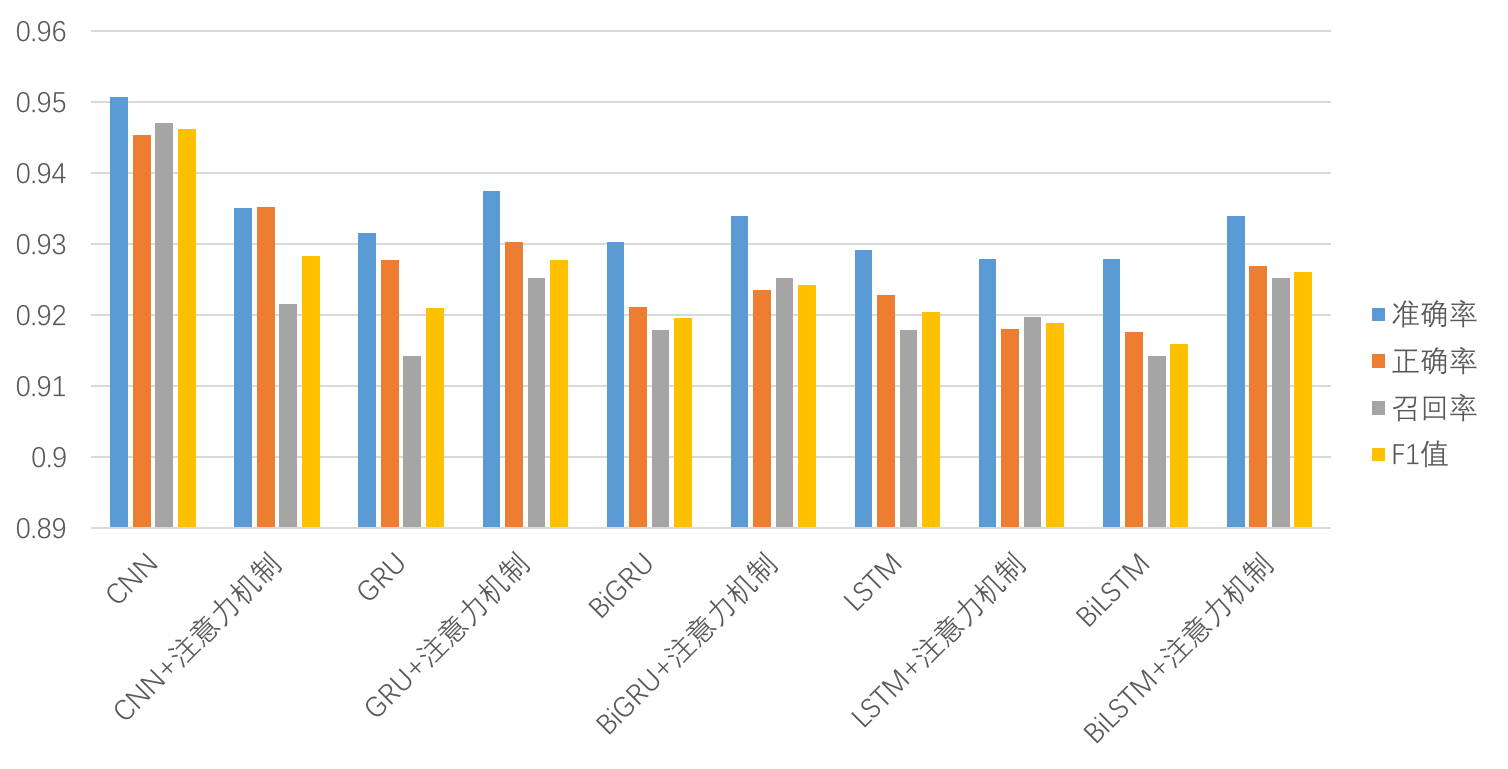
\includegraphics[width=\textwidth]{img/exp_context_emo_tri_result_bar.png}
  \caption{面向“开心”、“悲伤”和“愤怒”的三分类器模型性能}
  \label{fig:exp_context_emo_tri_result_bar}
\end{figure}

对于表中的四个指标,均由CNN达到最好的效果。对于F1值,排第二和第三的分别是CNN配合注意力机制以及GRU配合注意力机制,两者和CNN的F1值差距明显(约0.0179)。对于准确率,第二的GRU配合注意力机制和第三的CNN配合注意力机制的数值接近,但都和CNN有一定差距(约0.132)。对于正确率,第二为CNN配合注意力机制,数值明显低于CNN(差距约0.0102)。对于召回率,由GRU配合注意力机制、BiGRU配合注意力机制、BiLSTM配合注意力机制并排第二,与CNN的召回率差距明显(约0.0219)。

另外,虽然添加注意力机制对CNN的性能依然没有正面作用,但GRU、BiGRU和BiLSTM在添加注意力机制后都有较明显的提升,显示注意力模型有效捕捉此问题背后的某种语言特征。

\subsubsection{面向“其他”和“不是其他”二分类的模型性能分析}
\label{sssec:exp_context_emo_b_base}

对于面向三轮对话的“其他”和“不是其他”二分类问题,表~\ref{tab:exp_context_emo_b_result}和图~\ref{fig:exp_context_emo_b_result_bar}显示各个模型在测试集上的性能。注意表中的正确率、召回率、F1值同样对应“其他”一类的指标。

\begin{table}[htb]
  \centering
  \begin{minipage}[t]{\linewidth}
  \caption{面向“其他”和“不是其他”的二分类模型性能}
  \label{tab:exp_context_emo_b_result}
    \begin{tabularx}{\linewidth}{X|llll}
    \toprule[1.5pt]
    & 准确率 & 正确率 & 召回率 & F1值 \\
    \hline
    CNN & 0.9227 (2) & 0.9634 (3) & 0.9448 (2) & 0.9540 (2) \\ % f_b_cnn_ek_1554620963 
    CNN+注意力机制 & 0.9116 (7) & 0.9560 (9) & 0.9391 (3) & 0.9475 (7) \\ % f_b_cnn_ek_1554620537 
    \hline
    GRU & 0.9074 (9) & \bf 0.9670 (1) & 0.9224 (9) & 0.9442 (9) \\ % f_b_gru_ek_1554547645 
    GRU+注意力机制 & \bf 0.9230 (1) & 0.9553 (10) & \bf 0.9540 (1) & \bf 0.9546 (1) \\ % f_b_gru_ek_1554561028 
    \hline
    BiGRU & 0.9134 (4) & 0.9630 (4) & 0.9339 (6) & 0.9482 (4) \\ % f_b_bgru_ek_1554547845 
    BiGRU+注意力机制 & 0.9152 (3) & 0.9624 (6) & 0.9367 (5) & 0.9494 (3) \\ % f_b_bgru_ek_1554561013 
    \hline
    LSTM & 0.9011 (10) & 0.9649 (2) & 0.9168 (10) & 0.9402 (10) \\ % f_b_lstm_ek_1554549276 
    LSTM+注意力机制 & 0.9121 (6) & 0.9567 (8) & 0.9391 (3) & 0.9478 (6) \\ % f_b_lstm_ek_1554554626 
    \hline
    BiLSTM & 0.9089 (8) & 0.9595 (7) & 0.9320 (8) & 0.9456 (8) \\ % f_b_blstm_ek_1554549287 
    BiLSTM+注意力机制 & 0.9131 (5) & 0.9627 (5) & 0.9337 (7) & 0.9480 (5) \\ % f_b_blstm_ek_1554553473 
    \bottomrule[1.5pt]
    \end{tabularx}
  \end{minipage}
\end{table}

对于F1值,GRU配合注意力机制达到最高数值的0.9546, 其次的CNN和BiGRU配合注意力机制
都和前者的数值接近(分别为0.9540和0.9494)。对于准确率,排名前三的模型同样依次是GRU配合注意力机制、CNN和BiGRU配合注意力机制,前两者数值比较接近(0.9230和0.9227),第三的数值(0.9152)则和前两者差距较明显。对于正确率,由GRU达到最好的性能(0.9670),其次的LSTM(0.9649)和CNN(0.9634)的性能也比较接近。 对于召回率,排名第一第二的依然是GRU配合注意力机制(0.9549)和CNN(0.9448),CNN配合注意力机制以及LSTM配合注意力机制并排第三(0.9391)。

虽然GRU配合注意力机制在三项指标上都排名第一,但其正确率却是各个模型中排名倒数第一。相对地,对正确率排名第一第二的LSTM和GRU,它们在另外三项指标上却都排名倒数第一第二。可见数据不均匀会影响模型的识别倾向,甚至出现模型只在个别指标上明显靠前但同时也其他指标上明显靠后的情况。

\begin{figure}[H]
  \centering
  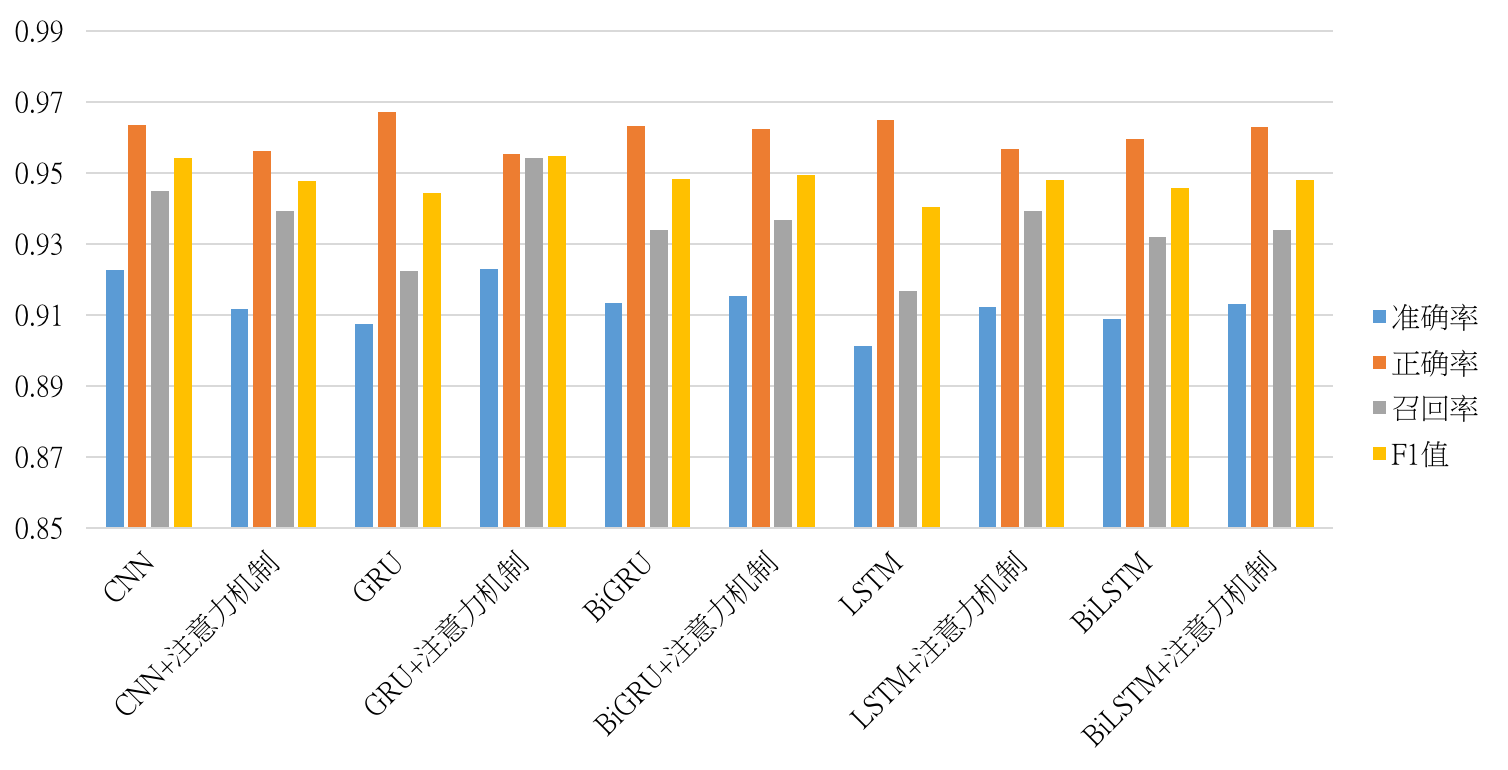
\includegraphics[width=\textwidth]{img/exp_context_emo_b_result_bar.png}
  \caption{面向“其他”和“不是其他”的二分类模型性能}
  \label{fig:exp_context_emo_b_result_bar}
\end{figure}

\subsubsection{面向三轮对话的情感识别系统的性能分析}

经过前面各章节的分析,我们已经对各个子分类问题中不同模型的性能有大致了解,接下来我们将研究由多组子分类器集成得出的情感识别系统的性能,并和比赛SemEval-2019任务三的参赛系统比较来评估我们系统的性能水平。

按照章节~\ref{sec:exp_context_emo_framework},我们的情感识别算法涉及三个子分类问题。对于和原问题相同的情感四分类问题,根据章节~\ref{sssec:exp_context_emo_0_base}的实验结果,我们采用CNN作为第一组分类器的模型。对于面向“开心”、“悲伤”和“愤怒”的三分类问题,按照章节~\ref{sssec:exp_context_emo_tri_base}的实验结果,我们同样选用CNN作为第二组分类器的模型。对于面向“其他”和“不是其他”的二分类问题,按照章节~\ref{sssec:exp_context_emo_b_base}的实验结果,我们采用GRU作为第三组分类器的模型。按照章节~\ref{ssec:exp_context_emo_model_training},我们基于选定的模型分别为每个分类器组训练5个分类器。

最后按照章节~\ref{sec:exp_context_emo_framework}中给出的识别流程,透过逐步结合各组分类器的投票结果得出三轮对话中最后一轮所表达的情感类别。对于系统中对第二、三组分类器需要配置的参数$thr_2$和$thr_3$,我们均设置为3。

\begin{table}[htb]
  \centering
  \begin{minipage}[t]{0.6\linewidth}
  \caption{SemEval-2019任务三前十名参赛系统性能} % 总参赛队伍165
  \label{tab:exp_context_emo_other_comp}
    \begin{tabularx}{\linewidth}{c|X|c}
    \toprule[1.5pt]
    排名 & 队伍名称 & F1值 \\
    \hline
    1 & PingAn GammaLab & 0.7959 \\
    2 & (无) & 0.7947 \\
    3 & NELEC & 0.7765 \\
    4 & SymantoResearch & 0.7731 \\
    5 & ANA & 0.7709 \\
    6 & CAiRE\_HKUST & 0.7677 \\
    7 & SNU\_IDS & 0.7661 \\
    8 & \bf THU\_HCSI & 0.7616 \\
    9 & (无) & 0.7608 \\
    10 & YUN-HPCC & 0.7588 \\
    \bottomrule[1.5pt]
    \end{tabularx}
  \end{minipage}
\end{table}

表~\ref{tab:exp_context_emo_other_comp}显示我们的系统和SemEval-2019任务三中其他参赛系统在测试集上最后一次提交的性能。注意表中的F1值为
针对“开心”、“悲伤”和“愤怒”的指标,即章节~\ref{ssec:exp_context_emo_eval_metric}中定义的$F_\mu$。在SemEval-2019任务三的最终测试阶段,参赛系统共165个,但官方只给出了各个参赛系统的F1值。表中仅显示排名前10(按照F1值排名)的参赛系统,其中队伍名称为THU\_HCSI对应我们当时提交的系统,排名第8。

另外,由于我们的算法中每一步的输出都可以作为一组预测结果,因此我们观察了每个中间结果在测试集上的性能。以下的系统由重新训练的子分类器组成,由于子分类器的训练存在随机性(参考章节~\ref{ssec:exp_context_emo_model_training}),因此和我们当时的参赛系统的F1值不同,但并不影响我们分析系统中每步决策的作用。

\begin{table}[htb]
  \centering
  \begin{minipage}[t]{0.6\linewidth}
  \caption{多分类器分层识别算法的中间结果和最终结果在测试集上的性能}
  \label{tab:exp_context_emo_ensemble_result}
    \begin{tabularx}{\linewidth}{X|cccc}
    \toprule[1.5pt]
    & 准确率 & 正确率 & 召回率 & F1值 \\
    \hline
    中间结果I & 0.9278 & 0.7360 & 0.7740 & 0.7545 \\
    中间结果II & 0.9281 & 0.7383 & \bf 0.7764 & 0.7569 \\
    \hline
    最终结果 & \bf 0.9299 & \bf 0.7474 & 0.7752 & \bf 0.7611 \\ 
    \bottomrule[1.5pt]
    \end{tabularx}
  \end{minipage}
\end{table}

表~\ref{tab:exp_context_emo_ensemble_result}中第一行“中间结果I”对应直接由一组情感四分类器(第一组分类器)进行多数投票的识别结果。第二行“中间结果II”是基于“开心”、“悲伤”和“愤怒”三分类器组(第二组分类器)的投票对原本被识别为这三个类别之一的样本重新进行分类的识别结果,可见四项指标都有所提升。再对比中间结果I和中间结果II的混淆矩阵(分别对应表~\ref{tab:exp_context_emo_conf_mat_1}和表~\ref{tab:exp_context_emo_conf_mat_2})可以发现4个样本的识别结果被正确修正,2个“愤怒”的样本被误判为“悲伤”,这显示了即使引入阈值$thr_2$来评估投票的可信度,由子分类器之间投票得出的识别结果依然会存在判断出错的情况,但整体上还是加强了对“开心”、“悲伤”和“愤怒”的区分能力。

表中最底一行的“最终结果”是基于“其他”和“不是其他”的二分类器组(第三组分类器)的投票结果尝试召回更多“其他”的样本,可见除了召回率有稍微下降,其他三项指标都有所提升,虽然准确率只稍微上升,但正确率的明显提升大大提高了最终的F1值。再对比中间结果II和最终结果的混淆矩阵(分别对应表~\ref{tab:exp_context_emo_conf_mat_2}和表~\ref{tab:exp_context_emo_conf_mat_3})可以发现11个“其他”的样本被正确召回,间接提高了“开心”、“悲伤”和“愤怒”的正确率$P_\mu$,但同时误判了1个原本正确的样本,故召回率$R_\mu$下降。同样地第三组分类器在引入阈值$thr_3$后依然会为识别结果带来错误的修改,但被正确召回的样本比错误的多,整体上对系统的识别结果也是起着正面的作用。

\begin{table}[]
  \centering
  \begin{minipage}[t]{0.54\linewidth}
  \caption{
    \label{tab:exp_context_emo_conf_mat_1}
    测试集上中间结果I对应的混淆矩阵
  }
  \begin{tabularx}{\linewidth}{c|c|cccc}
  \toprule[1.5pt]
  \multicolumn{2}{c|}{\multirow{2}{*}} & \multicolumn{4}{c}{预测标签}    \\
  \cline{3-6} 
  \multicolumn{2}{c|}{}
    & 其他 & 开心 & 悲伤 & 愤怒  \\
  \hline
  \multirow{4}{*}{真实标签}
    & 其他 & 4467 & 65 & 57 & 88 \\
    & 开心 & 82 & 196 & 4 & 2 \\
    & 悲伤 & 38 & 2 & 201 & 9 \\
    & 愤怒 & 47 & 1 & 3 & 247 \\
  \bottomrule[1.5pt]
  \end{tabularx}
  \end{minipage}
\end{table}

\begin{table}[]
  \centering
  \begin{minipage}[t]{0.54\linewidth}
  \caption{
    \label{tab:exp_context_emo_conf_mat_2}
    测试集上中间结果II对应的混淆矩阵
  }
  \begin{tabularx}{\linewidth}{c|c|cccc}
  \toprule[1.5pt]
  \multicolumn{2}{c|}{\multirow{2}{*}} & \multicolumn{4}{c}{预测标签}    \\
  \cline{3-6} 
  \multicolumn{2}{c|}{}
    & 其他 & 开心 & 悲伤 & 愤怒  \\
  \hline
  \multirow{4}{*}{真实标签}
    & 其他 & 4467 & 65 & 60 & 85 \\
    & 开心 & 82 & 197 & 4 & 1 \\
    & 悲伤 & 38 & 1 & 204 & 7 \\
    & 愤怒 & 47 & 1 & 5 & 245 \\
  \bottomrule[1.5pt]
  \end{tabularx}
  \end{minipage}
\end{table}

\begin{table}[]
  \centering
  \begin{minipage}[t]{0.54\linewidth}
  \caption{
    \label{tab:exp_context_emo_conf_mat_3}
    测试集上最终结果对应的混淆矩阵
  }
  \begin{tabularx}{\linewidth}{c|c|cccc}
  \toprule[1.5pt]
  \multicolumn{2}{c|}{\multirow{2}{*}} & \multicolumn{4}{c}{预测标签}    \\
  \cline{3-6} 
  \multicolumn{2}{c|}{}
    & 其他 & 开心 & 悲伤 & 愤怒  \\
  \hline
  \multirow{4}{*}{真实标签}
    & 其他 & 4478 & 60 & 57 & 82 \\
    & 开心 & 82 & 197 & 4 & 1 \\
    & 悲伤 & 39 & 1 & 203 & 7 \\
    & 愤怒 & 47 & 1 & 5 & 245 \\
  \bottomrule[1.5pt]
  \end{tabularx}
  \end{minipage}
\end{table}

接下来,我们分析一下选择面向“开心”、“悲伤”和“愤怒”三分类以及面向“其他”和“不是其他”二分类这两个子分类问题的合理性。首先对于面向“开心”、“悲伤”和“愤怒”的三分类问题,参考章节\ref{sssec:exp_context_emo_tri_base}可以发现我们的模型在该子问题上有很好的区分能力(F1值达到0.9462),其数值明显高于原本的四分类问题(对比章节\ref{sssec:exp_context_emo_0_base}中最高的F1值为0.7437),可见在引入类别“其他”后对F1值有较大影响,一方面是数据量的增加,另一方面说明模型同时区分“其他”和另外三个类别存在较明显的困难。另外,回顾章节\ref{sssec:exp_context_emo_0_base}、\ref{sssec:exp_context_emo_tri_base}和\ref{sssec:exp_context_emo_b_base}可以发现前两个子问题中F1值最高的都是CNN,而后者F1值最高的是GRU配合注意力机制,显示“其他”和另外三个类别背后的数学模型应该稍有不同。因此在第二步中我们以CNN重新对被识别为“开心”、“悲伤”和“愤怒”的样本进行区分,然后在第三步中以不同的模型来识别出原本没有被召回的“其他”的样本,以结合两种模型的识别能力。

对于为什么只召回“其他”的样本,而没有反过来召回“不是其他”的样本再进行三分类,这和各类别样本量的分布有关。“其他”的样本量在测试上明显多于另外三个类别的样本量,
如果尝试进一步召回“不是其他”的样本,系统会同时把更多“其他”的样本误判为“不是其他”,这就导致正确率$P_\mu$的下降显着大于召回率$R_\mu$的提升,从而导致核心指标$F_\mu$下降。而相反地从原本被识别为“开心”、“悲伤”和“愤怒”的样本中召回“其他”的样本,虽然会把部分原本识别正确的样本误判为“其他”,但会有较大概率召回更多正确的“其他”的样本,间接提高正确率$P_\mu$,因此我们选择召回更多“其他”的样本作为第三步的核心目标。

\subsection{错误分析}
\label{ssec:exp_context_emo_error_analysis}

本节中,我们将对系统错误识别的样本进行观察,分析其中的原因,从而对问题有更探入的了解,以及尝试给出下一步的改进方向。以下使用的例子均参照表~\ref{tab:semeval_2019_task3_error}。

\begin{table}[]
  \centering
  \begin{minipage}[t]{0.7\linewidth}
  \caption{
    \label{tab:semeval_2019_task3_error}
    测试集中被系统误判的样本例子
  }
  \begin{tabularx}{\linewidth}{c|c|l}
  \toprule[1.5pt]

   编号 & 类别 & 对话    \\
  \hline
  \multirow{3}{*}{1} & \multirow{3}{*}{开心} 
    &   (第一轮)用户甲: I'm in mood \\
    & & (第二轮)用户乙: ya need a hug ? :-) \\
    & & (第三轮)用户甲: yeah \\
  \hline
  \multirow{3}{*}{2} & \multirow{3}{*}{悲伤} 
    &   (第一轮)用户甲: I am \\
    & & (第二轮)用户乙: in your dreams \\
    & & (第三轮)用户甲: Haha Bite me! 
\includegraphics[height=1.5\fontcharht\font`\B]{img/emoji/speechless.png}
\includegraphics[height=1.5\fontcharht\font`\B]{img/emoji/speechless.png}
\includegraphics[height=1.5\fontcharht\font`\B]{img/emoji/speechless.png} \\
  \hline
  \multirow{3}{*}{3} & \multirow{3}{*}{愤怒} 
    &   (第一轮)用户甲: You are pig \\
    & & (第二轮)用户乙: so are you \\
    & & (第三轮)用户甲: You are dog \\
  \hline
  \multirow{3}{*}{4} & \multirow{3}{*}{其他} 
    &   (第一轮)用户甲: Wat u wanna knw? \\
    & & (第二轮)用户乙: i knw nothin :P \\
    & & (第三轮)用户甲: 
\includegraphics[height=1.5\fontcharht\font`\B]{img/emoji/lol.png}
\includegraphics[height=1.5\fontcharht\font`\B]{img/emoji/lol.png} \\
  \hline
  \multirow{3}{*}{5} & \multirow{3}{*}{开心} 
    &   (第一轮)用户甲: You cannot see my hair \\
    & & (第二轮)用户乙: I'm in your closet \\
    & & (第三轮)用户甲: 
\includegraphics[height=1.5\fontcharht\font`\B]{img/emoji/lol.png} \\
  \bottomrule[1.5pt]
  \end{tabularx}
  \end{minipage}
\end{table}


\begin{itemize}

\item {\bf 词组情感倾向识别}。参考例子1,第一轮中用户甲的“in mood”表示心情愉快,属于正向情感,第三轮中的“yeah”也略带正向情感,按照章节~\ref{ssec:exp_context_emo_multi_turn_analyse},应该得出样本情感标签为“开心”。然而“in mood”在训练集中主要以“not in mood”出现,且这些样本标签都是“悲伤”,显然系统未能正确识别“in mood”本身的情感倾向导致了识别错误,另外可以推测对于在训练集上没有出现过的词组也会有相同的问题。在章节~\ref{ssec:exp_irony_det_error_analysis}中相同,只能透过额外引入语言知识解决。

\item {\bf 对于同时出现多种情感的处理}。参考例子2,第三轮中用户甲的发言在字面上包含两种情感,首先是“Haha”表达偏向“开心”的情感,“Bite me!
\includegraphics[height=1.5\fontcharht\font`\B]{img/emoji/speechless.png}”则带有鄙视和不满的意思,倾向于“悲伤”。按照章节~\ref{ssec:exp_context_emo_multi_turn_analyse}的分析,应以后半“悲伤”的情感为主。然而我们选用的CNN模型中,CNN的序列输出以最大池整合为一个固定长度的向量,即模型没有考虑情感出现的先后顺序,而是直接保留了字面上情感最强烈的内容,这也显示对语言模式的了解有助于模型的设计。

\item {\bf 理解比喻修辞}。参考例子3,用户甲在第一轮和第三轮中都在以比喻的修辞辱骂用户乙,然而系统从字面意思上未能识别出其情感倾向于“愤怒”。首先,在训练集上确实存在“be a pig”且大部分的标注都为“愤怒”,理论上机器学习算法可以学习出“be a pig”带有表达“愤怒”的性质。但数据中没有包含“be a dog”的样本,那么如果算法未能关联“pig”和“dog”就不可能识别出“be a pig”的情感属性。而从语言的角度来看,解决这个问题的本质是识别出比喻的使用,并且理解其真实想表达的意思,这就回归到上一章节中对修辞手法进行建模的问题。

\item {\bf 语料中情感标注的不一致}。参考例子4,第三轮中用户甲的发言仅包含两个大笑的表情符“
\includegraphics[height=1.5\fontcharht\font`\B]{img/emoji/lol.png}”,而前两轮的文本内容则偏向中性,我们有理由认为这个样本应该标记为“开心”,然而组织者给出的标注为“其他”。再参考例子5,第三轮中用户甲的发言同样仅包含大笑的表情符“
\includegraphics[height=1.5\fontcharht\font`\B]{img/emoji/lol.png}”,而前两轮的文本内容同样偏向中性,但标注为“开心”。假如我们对例子4的情感判断正确,那就说明数据集内部对情感标注的标准存在不一致,这一方面会对模型的学习造成混淆,另一方面也会对系统评估带来影响。

\end{itemize}

\section{本章小结}

在本章中我们提出了一种多通道分类模型,用于研究面向三轮对话的情感识别,以结合各轮发言的信息。基于该模型,我们同时提出了一个多分类器分层情感识别算法,并用于国际比赛SemEval-2019任务三的情感识别问题,参赛结果显示我们系统的性能在165个参赛系统中排名前十。以此比赛为基础,我们进一步观察了我们的多分类器分层情感识别算法的性能表现,透过对算法的中间结果进行分析,解释了我们算法中每一步对整个算法的作用,同时验证了我们的算法设计的合理性。最后我们对被系统错误识别的样本进行分析,指出系统的不足之处并给出对应的改进方向。


